\section{Methoden}
	
	Dieser Abschnitt beschäftigt sich mit dem Aufbau der beiden Schaltkreise, sowie auch den Unsicherheiten welche bei der Messung auftreten.
	
	\subsection{Aufbau}
			
		\subsubsection{Serienresonanzkreis}
			
			\begin{figure}[ht]
				\centering
				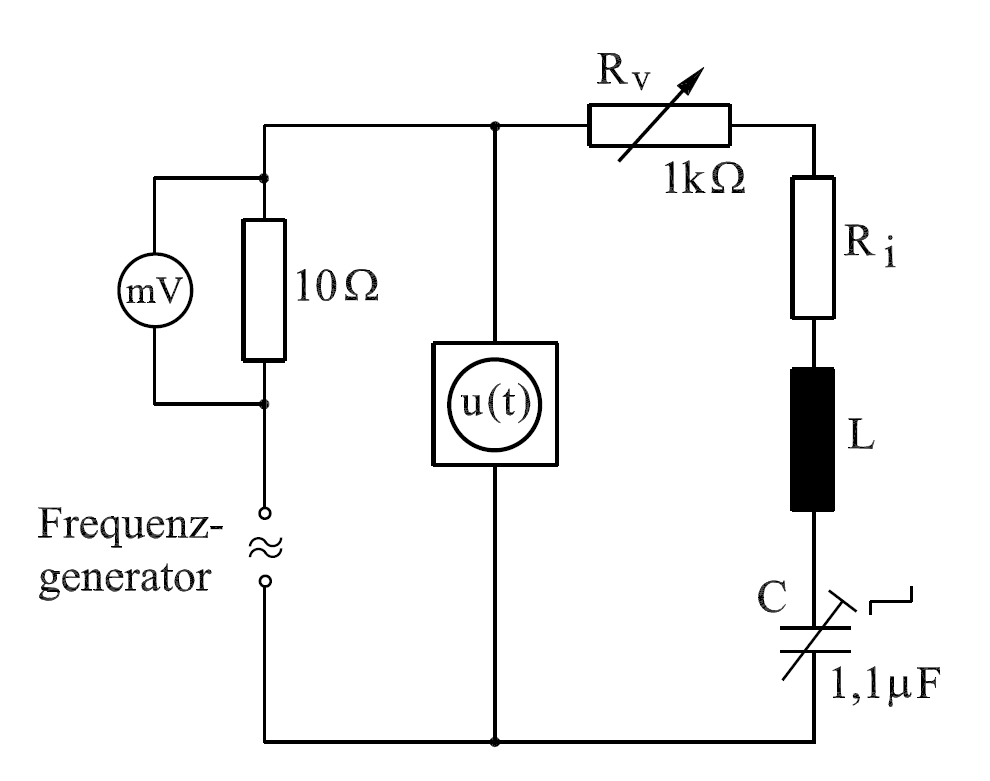
\includegraphics[width=0.55\textwidth]{auswertung/Serienresonanz.PNG}
				\caption{Schaltskizze für den Aufbau des Serienresonanzkreises.\cite{WWU}}
				\label{fig:SerienResonanzSkizze}	
			\end{figure}
			
			Für den Serienresonanzkreis wird der in Abb. \ref{fig:SerienResonanzSkizze} dargestellte Aufbau verwendet.
			Zu erkennen sind ein Frequenzgenerator, ein \SI{10}{\ohm} Widerstand, an dem ein Multimeter zur Messung der Spannung anliegt, ein Oszilloskop u$(t)$, welches parallel zu der Reihenschaltung von Kondensator $C$, Spule $L$ mit Innenwiderstand $R_\text{i}$ und einem bis zu \SI{1}{\kilo\ohm} regulierbaren Widerstand $R_\text{v}$ geschaltet ist.
			Der Frequenzgenerator dient als Wechselstromquelle, welcher auf eine feste Frequenz und Spannung eingestellt werden soll.
			 
		\subsubsection{Parallelresonanzkreis}
			
			\begin{figure}[ht]
				\centering
				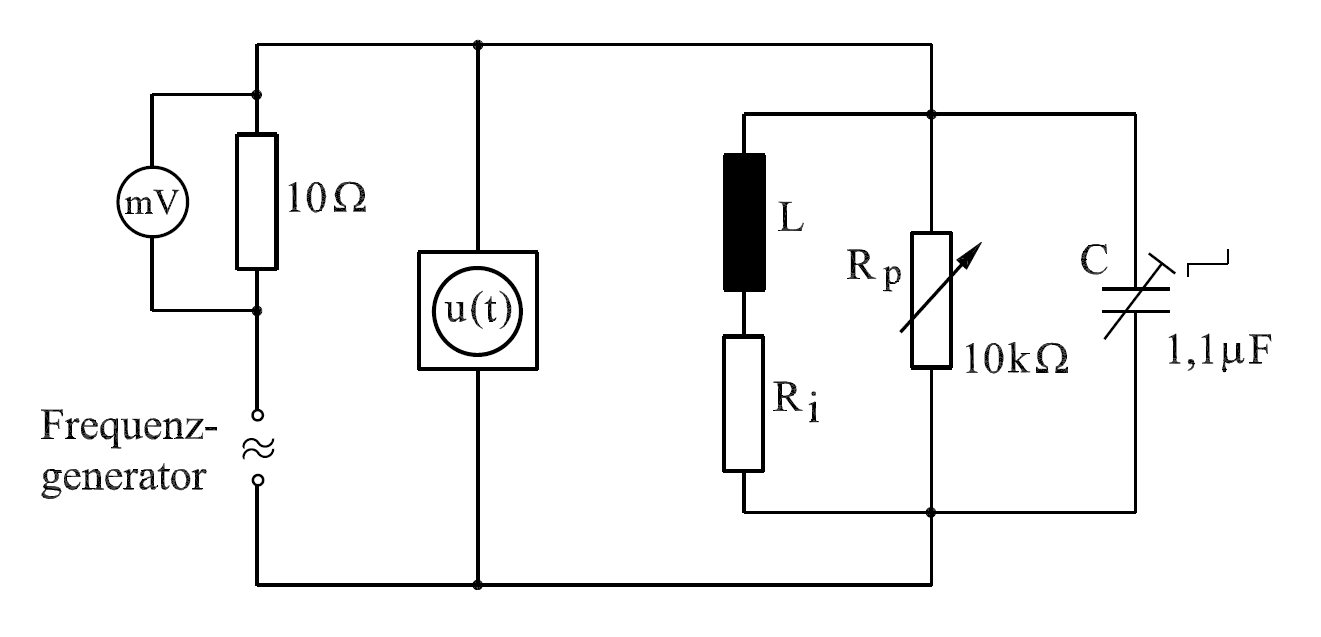
\includegraphics[width=0.7\textwidth]{auswertung/Parallelresonanz.PNG}
				\caption{Schaltskizze für den Aufbau des Parallelresonanzkreises.\cite{WWU}}
				\label{fig:ParallelResonanzSkizze}	
			\end{figure}
			
			Der in Abb. \ref{fig:ParallelResonanzSkizze} dargestellte Schaltkreis für den Parallelresonanzkreis unterscheidet sich von dem Serienschaltkreis lediglich um die Parallelschaltung von (einer kleineren) Spule $L$ mit Innenwiderstand $R_\text{i}$, Kondensator $C$ und einem bis zu \SI{10}{\kilo\ohm} regulierbaren Widerstand $R_\text{p}$. 
			Dieser Block ist wie auch zuvor parallel zu dem Oszilloskop geschaltet.
			Hier wird die selbe Frequenz, wie auch für den Serienresonanzkreis verwendet, jedoch eine höhere Spannung.

	\subsection{Unsicherheiten} 

		Die bei diesem Versuch auftretenden Unsicherheiten setzen sich aus der Unsicherheit für den Kondensator $u_\text{c}$, für die digitale Anzeige des Multimeters und des Oszilloskops $u_\text{digital}$, sowie der Unsicherheit des \SI{10}{\ohm} Widerstandes von $0,5\%$ (nach den angegebenen Farbcodes\cite{widerstand}). 
		Weitere Angaben, wie die Maße der großen Spule\footnote{Diese sind dem Laborbuch zu entnehmen}, bei denen keine Unsicherheit angegeben war, werden als absolut angenommen. 
		Die Berechnung der kombinierten Unsicherheiten erfolgt nach GUM und ist im Anhang aufgeführt.

\section{Durchführung und Datenanalyse}

	Zur Bestimmung der Resonanzkurve $I(f)$, wird die Stromstärke $I$ in den Schaltkreisen über die gemessenen Spannung $U$ und dem \SI{10}{\ohm} Widerstand ermittelt.
	Dazu dient $I = U/R$.
	Die verwendete Frequenz der Wechselstromquelle für beide Schwingkreise betrug \SI{1000}{\hertz}.
	Für die Eingangspannungen wurden für den Serienresonanzkreis \SI{2}{\volt} und \SI{5}{\volt} für den Parallelresonanzkreis verwendet.
	Es wurden für verschiedene Widerstände $R_\text{v}$ (Serie, mit \SI{0}{\ohm}, \SI{200}{\ohm} und \SI{500}{\ohm}) und $R_\text{p}$ (parallel, mit $\infty$ \si{\ohm}, \SI{2}{\kilo\ohm} und \SI{10}{\kilo\ohm}) Messungen in Abhängigkeit der Kapazität des Kondensators $C$ durchgeführt. 
	Dabei sind die aufgelisteten Widerstände solche, für die eine Messung durchgeführt werden sollte.
	Die eigentlichen Widerstände welche für diesen Versuch verwendet wurden waren, nach der Messung mit dem Multimeter, \SI{0,3}{\ohm}, \SI{200,1}{\ohm} und \SI{500,3}{\ohm} für den Serienresonanzkreis und $\infty$ \si{\ohm}, \SI{2,001}{\kilo\ohm} und \SI{9,88}{\kilo\ohm} für den Parallelresonanzkreis.
	Aus der Messreihe ergaben sich die in den Abb. \ref{fig:reihe0} bis \ref{fig:parallel10k} dargestellten Resonanzkurven\footnote{Die Fits wurden von dem Programm SciDavis berechnet, dazu wurden die Unsicherheiten der Auslenkung und die Methode der kleinsten Quadrate herangezogen} in Abhängigkeit der Kapazität $C$ (Serie) bzw. deren Kehrwert (Parallel). 
	\begin{figure}[ht]
		\centering
		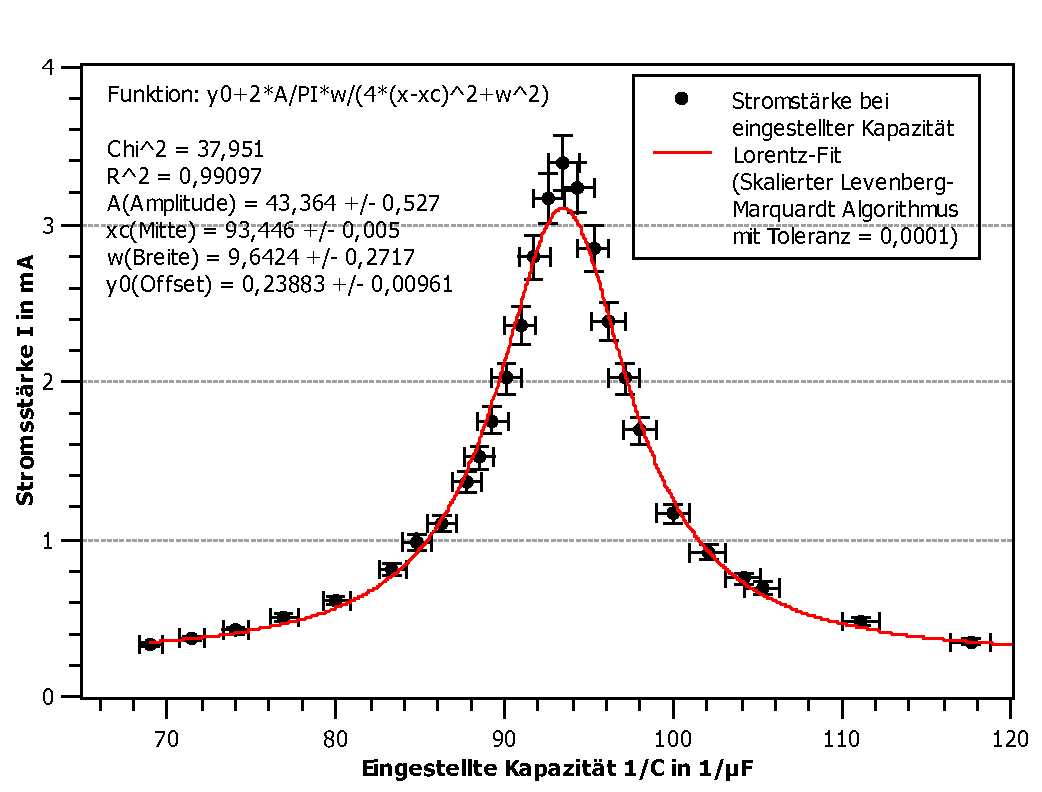
\includegraphics[width=0.7\textwidth]{auswertung/Reihe-0ohm(algo).pdf}
		\caption{Dieses Diagramm stellt die Resonanzkurve bei einem Serienresonanzkreis in Abhängigkeit des Kehrwerts der Kapazität bei einem Widerstand $R_\text{v}$ von \SI{0,3}{\ohm} dar. Es wurde aufgrund des Verlaufs ein Lorentz-Fit verwendet.}
		\label{fig:reihe0}	
	\end{figure}
	\begin{figure}[ht]
		\centering
		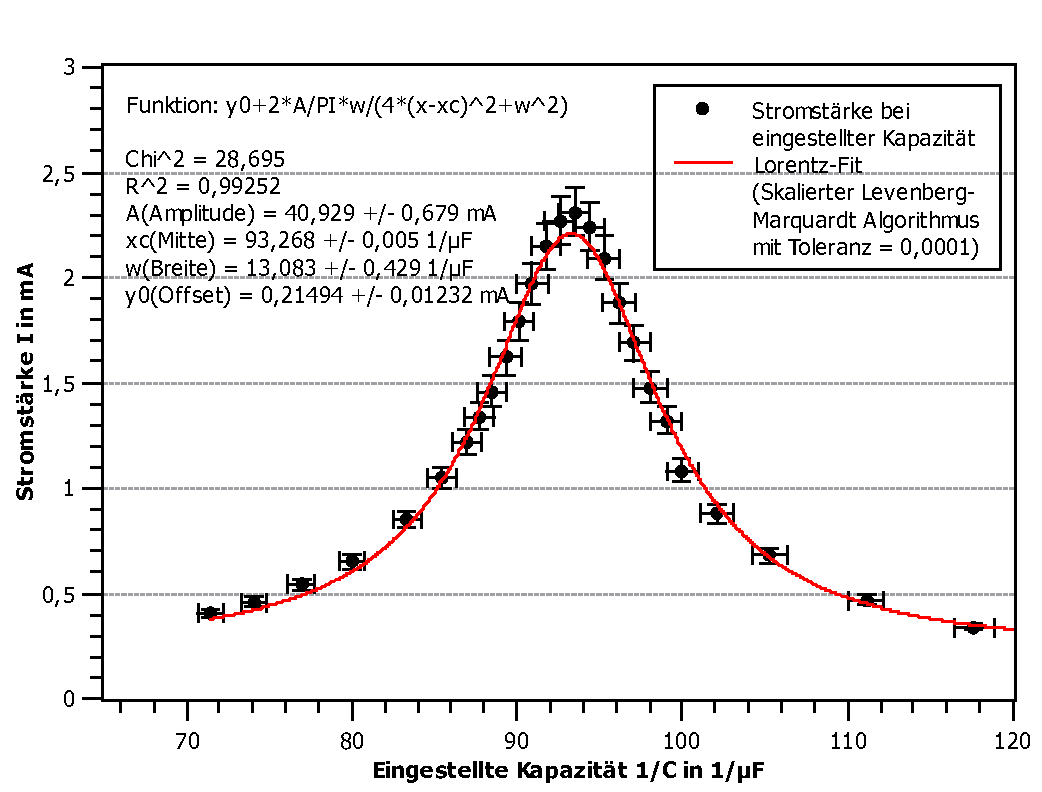
\includegraphics[width=0.7\textwidth]{auswertung/Reihe-200ohm(algo).pdf}
		\caption{Dieses Diagramm stellt die Resonanzkurve bei einem Serienresonanzkreis in Abhängigkeit des Kehrwerts der Kapazität bei einem Widerstand $R_\text{v}$ von \SI{200,1}{\ohm} dar. Es wurde aufgrund des Verlaufs ein Lorentz-Fit verwendet.}
		\label{fig:reihe200}	
	\end{figure}
	\begin{figure}[ht]
		\centering
		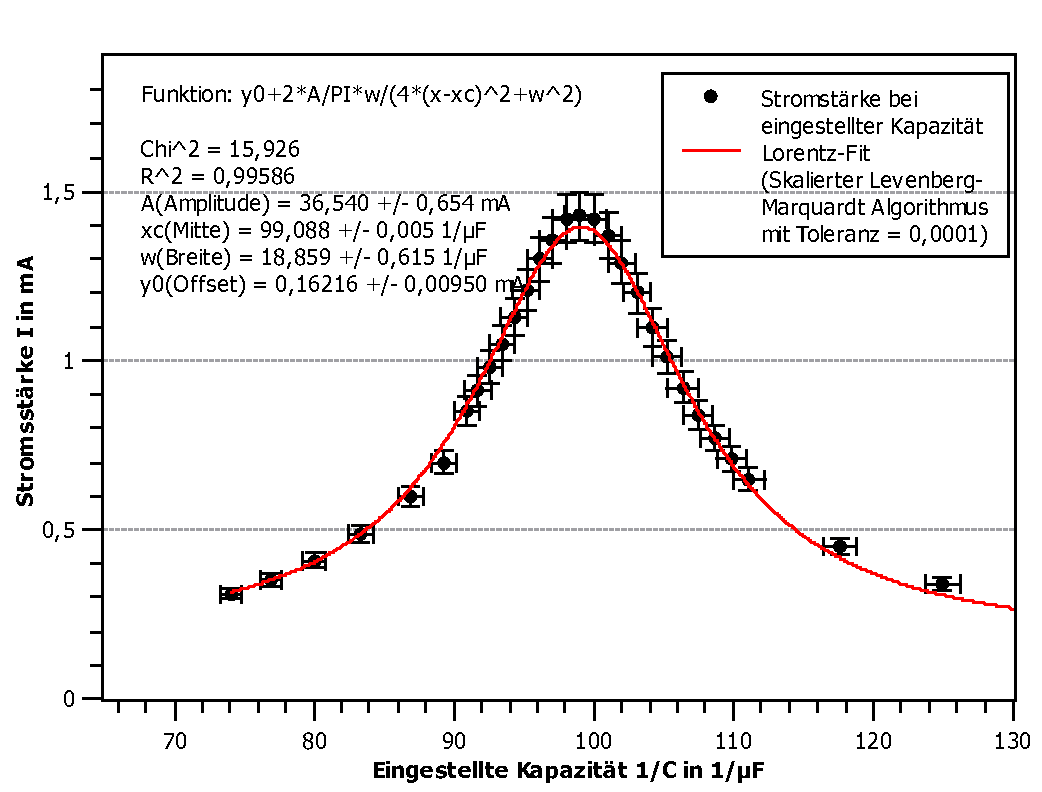
\includegraphics[width=0.7\textwidth]{auswertung/Reihe-500ohm(algo).pdf}
		\caption{Dieses Diagramm stellt die Resonanzkurve bei einem Serienresonanzkreis in Abhängigkeit des Kehrwerts der Kapazität bei einem Widerstand $R_\text{v}$ von \SI{500,3}{\ohm} dar. Es wurde  aufgrund des Verlaufs ein Lorentz-Fit verwendet.}
		\label{fig:reihe500}	
	\end{figure}
	\begin{figure}[ht]
		\centering
		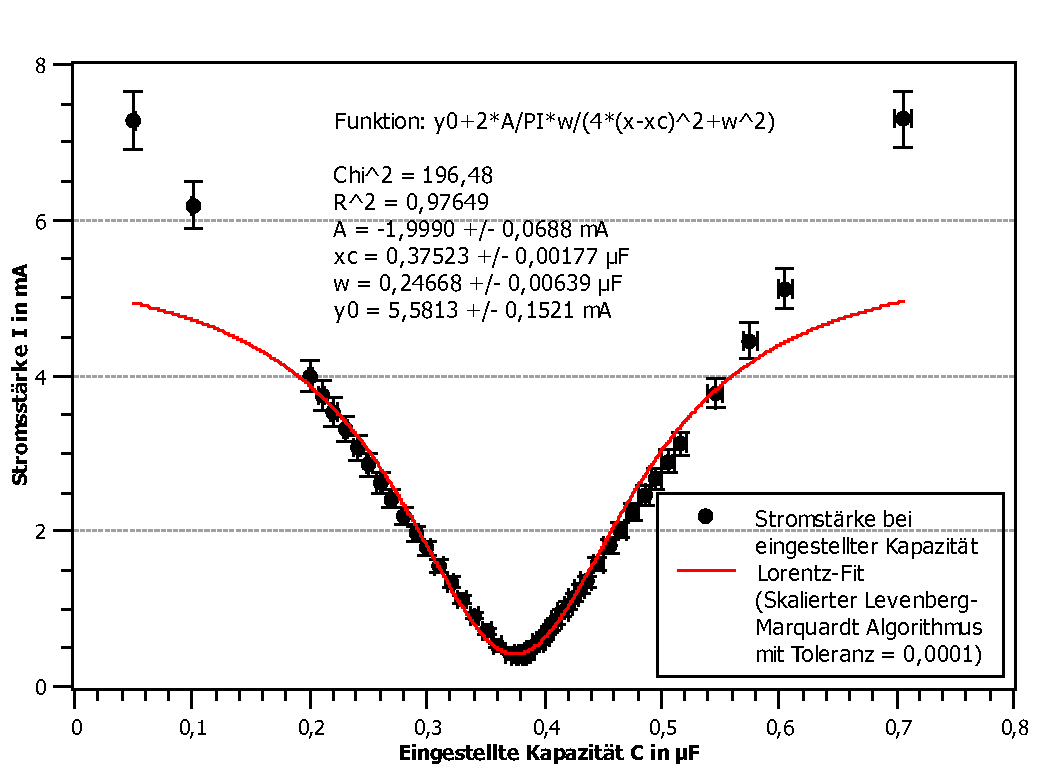
\includegraphics[width=0.7\textwidth]{auswertung/Parallel-infohm(algo).pdf}
		\caption{Dieses Diagramm stellt die Resonanzkurve bei einem Serienresonanzkreis in Abhängigkeit der Kapazität bei einem Widerstand $R_\text{p}$ von $\infty$ \si{\ohm} dar. Es wurde  aufgrund des Verlaufs ein Lorentz-Fit verwendet.}
		\label{fig:parallelinf}	
	\end{figure}
	\begin{figure}[ht]
		\centering
		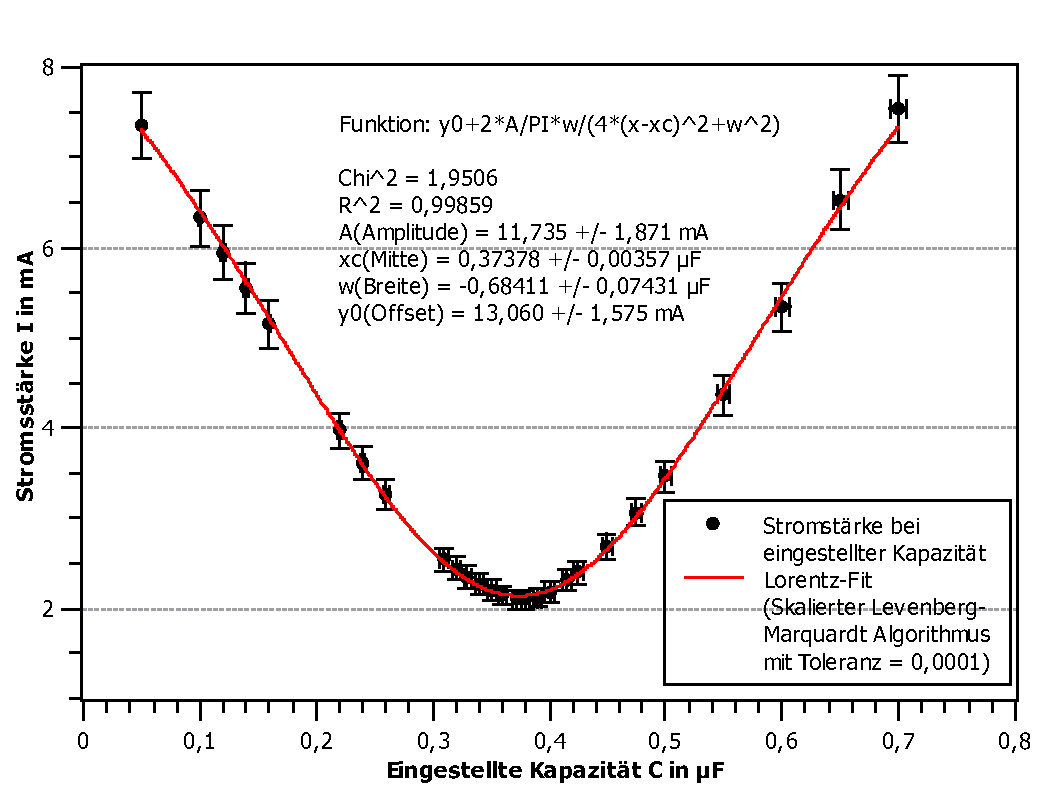
\includegraphics[width=0.7\textwidth]{auswertung/Parallel-2kohm(algo).pdf}
		\caption{Dieses Diagramm stellt die Resonanzkurve bei einem Serienresonanzkreis in Abhängigkeit der Kapazität bei einem Widerstand $R_\text{p}$ von \SI{2,001}{\kilo\ohm} dar. Es wurde aufgrund des Verlaufs ein Lorentz-Fit verwendet.}
		\label{fig:parallel2k}	
	\end{figure}
	\begin{figure}[ht]
		\centering
		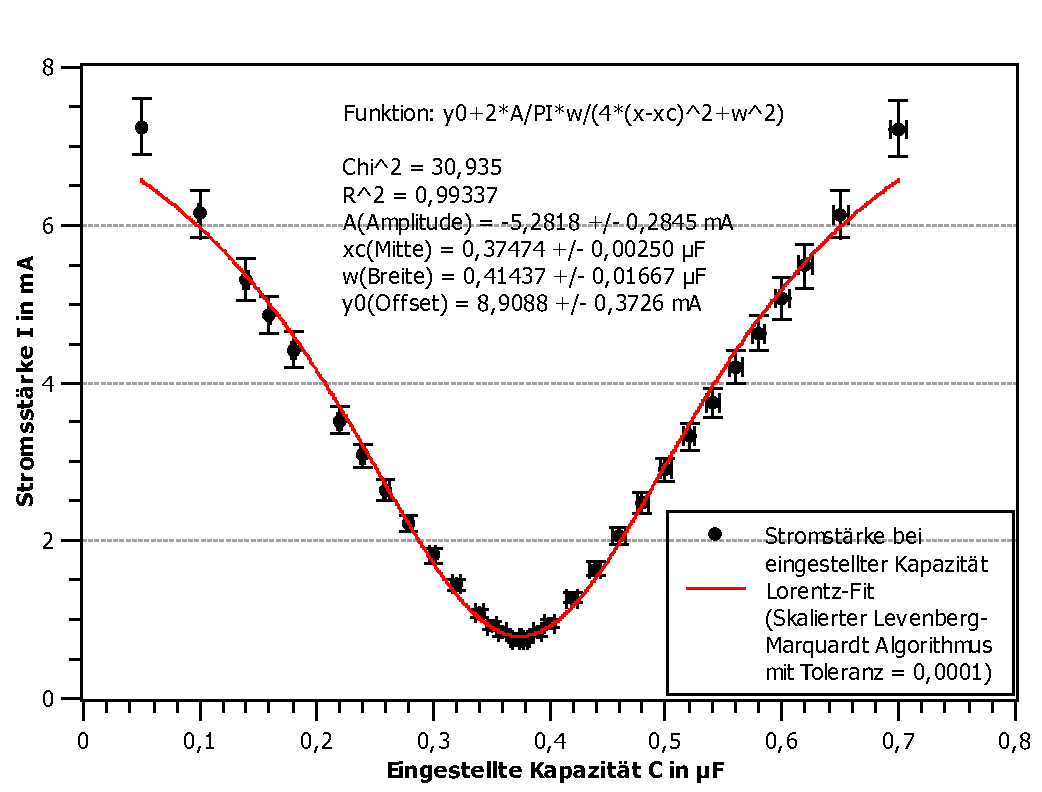
\includegraphics[width=0.7\textwidth]{auswertung/Parallel-10kohm(algo).pdf}
		\caption{Dieses Diagramm stellt die Resonanzkurve bei einem Serienresonanzkreis in Abhängigkeit der Kapazität bei einem Widerstand $R_\text{p}$ von \SI{9,88}{\kilo\ohm} dar. Es wurde aufgrund des Verlaufs ein Lorentz-Fit verwendet.}
		\label{fig:parallel10k}	
	\end{figure}	
	Durch diese Diagramme lassen sich die Induktivitäten der verwendeten Spulen bestimmen.
	Dazu dient folgender Zusammenhang, welcher aus der Impedanz $Z$ folgt:
	\begin{align}
		Z_\text{Serie} &= R_i + i\left(\omega L - \frac{1}{\omega C} \right) \\
		Z_\text{Parallel} &= \left( \frac{1}{R_i} + \frac{1}{i\omega L} + i\omega C\right)^{-1} \\
		\Rightarrow L &= \frac{1}{\omega_0^2 C}.
	\end{align}
	Dabei ist $R_i$ der Innenwiderstand der Spule, $L$ die Induktivität dieser und $C$ die Kapazität des Kondensators.	
	In Tab. \ref{tab:L} sind die berechneten Induktivitäten, wie auch die Kapazitäten bei denen die Resonanzfrequenz $\omega_0$ bei \SI{1000}{\hertz} bzw. der Kreisfrequenz \SI{6283,19}{\s^{-1}} liegt, dargestellt.	
	\begin{table}
		\caption{Diese Tabelle stellt die ermittelten Induktivitäten für die große Spule bei dem Serienresonanzkreis und der kleineren beim Parallelresonanzkreis in Abhängigkeit von der Kapazität $C$ (Serie) des Kondensators bzw. ihrem Kehrwert (Parallel).}
		\label{tab:L}
		\centering
		\begin{tabular}{c|c|c}
			$R_\text{v}$ & 1/C & Induktivität $L$ \\
			\hline
			\SI{0,3}{\ohm} & \SI{93,446+-0,005}{\micro\farad} & \SI{2,3670+-0,0001}{\henry} \\
			\SI{200,1}{\ohm} & \SI{93,268+-0,005}{\micro\farad} & \SI{2,3625+-0,0001}{\henry} \\ 
			\SI{500,3}{\ohm} & \SI{99,088+-0,005}{\micro\farad} & \SI{2,5099+-0,0001}{\henry} \\ 
		\end{tabular}
		\begin{tabular}{c|c|c}
			$R_\text{p}$ & $C$ & Induktivität $L$ \\
			\hline
			$\infty$ \si{\ohm} & \SI{0,375+-0,002}{\micro\farad} & \SI{0,0675+-0,0003}{\henry} \\
			\SI{2,001}{\kilo\ohm} & \SI{0,375+-0,003}{\micro\farad} & \SI{0,0676+-0,0005}{\henry} \\ 
			\SI{9,88}{\kilo\ohm} & \SI{0,374+-0,004}{\micro\farad} & \SI{0,0678+-0,0006}{\henry} \\
		\end{tabular}
	\end{table}
	Neben der Messung der Spannung wurde zudem der Spannungsabfall über das Oszilloskop an verschiedenen Stellen im Serienkreis bei der Resonanzfrequenz betrachtet.
	Diese Spannungsabfälle sind in Tab. \ref{tab:Abfall} verzeichnet. 
	\begin{table}
		\caption{In dieser Tabelle sind die gemessenen Spannungsabfälle so wie auch die ermittelten gegenüber gestellt. Zusätzlich wurden die Spannungsabfälle an dem Widerstand $R_\text{v}$ gemessen, diese sind jedoch nicht vergleichbar.}
		\label{tab:Abfall}
		\centering
		\begin{tabular}{c|c|c|c}
			Spannung & bei \SI{0,3}{\ohm} & bei \SI{200,1}{\ohm} & bei \SI{500,3}{\ohm}\\
			\hline
			$U_C$ (gemessen) & \SI{21,40+-0,02}{\volt} & \SI{32,06+-0,02}{\volt} & \SI{52,00+-0,02}{\volt} \\
			$U_C$ (ermittelt) & \SI{33,338+-0,508}{\volt} & \SI{26,377+-0,455}{\volt} & \SI{20,071+-0,344}{\volt} \\
			\hline
			$U_L$ (gemessen)  & \SI{25,20+-0,02}{\volt} & \SI{32,10+-0,02}{\volt} & \SI{51,20+-0,02}{\volt} \\
			$U_L$ (ermittelt)  & \SI{33,338+-0,237}{\volt} & \SI{26,377+-0,184}{\volt} & \SI{20,071+-0.136}{\volt} \\
		\end{tabular}
	\end{table}

\section{Diskussion}

	Um auf die Hypothese, dass die Resonanzkurven die Form einer Lorentzfunktion besitzen, zurückzugreifen, lässt sich dies eindeutig durch die Diagramme \ref{fig:reihe0} bis \ref{fig:parallel10k} bestätigen.
	Abgesehen von den Randwerten liegen die Lorentz-Fits nämlich nahezu alle innerhalb von einer Standardunsicherheit der Messwerte.
	Die ermittelten Induktivitäten der beiden Spulen, welche über die einzelnen Resonanzkurven und dem Verlustwiderstand bestimmt wurden, wirken recht realistisch.
	Werte im Bereich von \SI{2}{\henry} sind für Spulen recht groß, jedoch handelte es sich hierbei um eine Spule von großem Ausmaß, weswegen dieser Wert akzeptiert wird.
	Lediglich dass der Wert über die \SI{500}{\ohm}-Resonanzkurve ein wenig stärker von den anderen beiden ermittelten Induktivitäten für dieselbe Spule abweicht, geht gegen die Erwartung, dass die Induktivität für dieselbe Spule gleich bleibt.
	Für die kleinere Spule liegen alle Werte innerhalb von einer Standardunsicherheit voneinander.
	Bei den Spannungsabfällen muss aufgrund der deutlichen Abweichungen und dem antiproportionalen Verhalten von Mess- und ermittelten Werten ein Fehler aufgetreten sein, wo genau dieser liegt ist nicht ersichtlich. 